\documentclass[]{spie}  %>>> US letter paper

\renewcommand{\baselinestretch}{1.0}

\usepackage{amsmath,amsfonts,amssymb}
\usepackage{graphicx}
\usepackage{booktabs}
\usepackage[colorlinks=true, allcolors=blue]{hyperref}

\graphicspath{{figures/}}

\title{Are magnetic nanoparticles visible in CT? A simulation study of SPION
detectability with energy-integrating and photon-counting detectors}

\author[a]{Andreas Maier}
\author[b]{Stefan Lyer}
\author[b]{Lukas Heinen}
\author[b]{Rainer Tietze}
\affil[a]{Pattern Recognition Lab, Friedrich-Alexander-Universit\"at Erlangen-N\"urnberg, Germany}
\affil[b]{SEON -- Section of Experimental Oncology and Nanomedicine, Department of
Otorhinolaryngology, Universit\"atsklinikum Erlangen / FAU, Germany}

\authorinfo{Send correspondence to A.M.: E-mail: andreas.maier@fau.de}

\pagestyle{empty}
\setcounter{page}{1}

\begin{document}
\maketitle

\begin{abstract}
Superparamagnetic iron-oxide nanoparticles (SPIONs) are increasingly used for
magnetic drug targeting, hyperthermia, and cell tracking, yet it is rarely asked
whether the iron they deposit is actually visible in a computed tomography (CT)
scan. We study this question by simulation. Starting from a real magnetite SPION
formulation, we build a physically grounded \emph{delivered-mass} dose model: a
fixed particle mass is spread through an $8\,\mathrm{cm}^3$ tumor, which for the
reference $6\,\mathrm{mg}$ dose leaves only $\sim\!0.54\,\mathrm{mg\,Fe/ml}$ --
about an order of magnitude below iodine CT enhancement. Using the CONRAD
framework we simulate a rabbit-scale phantom imaged with a polychromatic
$90\,\mathrm{kVp}$ C-arm spectrum at $70{,}000$ photons per pixel, and run a
factorial experiment over iron dose, detector type (energy-integrating, EID, vs.\
three-bin photon-counting, PCD), and water beam-hardening correction, scoring
detectability by iron contrast ($\Delta$HU) and contrast-to-noise ratio (CNR)
against the Rose criterion. We find that the reference dose sits \emph{right at}
the detection limit: iron contrast is only $3.4\,$HU (EID) to $4.7\,$HU (PCD) with
CNR $\approx 5$. The detection threshold is $\approx 0.54\,\mathrm{mg\,Fe/ml}$ and
is essentially unchanged by detector type or beam-hardening correction; a
matched-filter PCD gain of $\sim\!1.3\times$ appears only at twice the dose, once
the photon-starved low-energy bin carries enough counts. Lowering the tube voltage
helps and hardening filters hurt, consistent with the photoelectric origin of iron
contrast. SPIONs are therefore borderline-visible at realistic loading -- a result
with direct consequences for image-guided nanoparticle therapy.
\end{abstract}

\keywords{SPION, iron oxide nanoparticles, computed tomography, photon counting,
detectability, contrast-to-noise ratio, simulation, CONRAD}

\section{INTRODUCTION}
\label{sec:intro}

Superparamagnetic iron-oxide nanoparticles (SPIONs) have become a workhorse of
nanomedicine. They are steered by magnetic fields for local drug delivery, heated
for hyperthermia, and used as labels for cell tracking. A natural clinical
question follows: once these particles have accumulated in a target region, can we
simply \emph{see} them in a routine CT scan? The answer matters for dose planning,
for interpreting incidental findings, and for image-guided delivery, where one
would like to confirm that particles reached the target without an additional
imaging modality.

At first sight iron looks promising: it is denser and higher in atomic number than
soft tissue. The difficulty is the amount. At biologically realistic loading the
delivered iron mass is small. If a few milligrams of particles are distributed
through a cubic-centimeter-scale tumor, the resulting iron concentration is on the
order of tenths of a milligram per millilitre -- roughly ten times below the iodine
concentrations that produce comfortable CT enhancement. Whether that little iron
rises above image noise is not obvious, and it is exactly the kind of question a
careful simulation can answer before any animal is scanned.

Despite a large literature on SPIONs and a parallel surge of interest in
photon-counting CT, there is little quantitative simulation of SPION CT
detectability across modern detectors. We address this gap. Our contributions are:
(i) a physically grounded \emph{delivered-mass} dose model tied to a real magnetite
SPION formulation, which converts a formulation concentration into an in-tumor iron
concentration; (ii) a factorial detectability study that compares an
energy-integrating detector (EID) with a multi-bin photon-counting detector (PCD),
with and without beam-hardening correction; and (iii) reported detection thresholds
in $\mathrm{mg\,Fe/ml}$, scored by both iron contrast ($\Delta$HU) and
contrast-to-noise ratio (CNR) against the Rose criterion. The entire pipeline is
built on the open-source CONRAD framework\cite{Maier2013}, and the code, figures,
and intermediate results are public for audit.

We deliberately keep the paper honest: if the realistic dose turns out to be
borderline, that is itself a useful and publishable finding for anyone planning to
image nanoparticle therapy with CT.

\section{MATERIALS AND METHODS}
\label{sec:methods}

We first fix the dose model, then the phantom, then the X-ray simulation,
reconstruction, and the detectability metrics. Each choice is made to keep the
$c_{\mathrm{Fe}}=0$ case identical to background, so that any measured contrast is
attributable to iron alone.

\subsection{Nanoparticle and delivered-mass dose model}
The formulation we ground on is a real polyacrylic-acid (PAA)-coated magnetite
($\mathrm{Fe_3O_4}$) SPION suspension\cite{Heinen2026}, with iron-oxide cores of
$\sim\!8$ and $\sim\!12\,\mathrm{nm}$ that assemble into hydrodynamic clusters of
$\sim\!70$--$250\,\mathrm{nm}$. It is worth being explicit about how the particles
are quantified, because the particle-versus-iron distinction is easy to conflate.
The reference article characterizes the suspension by its \emph{iron} concentration
in $\mathrm{mg\,Fe/ml}$, measured by ICP-MAES on acid-digested particles, over a
working range of $1$--$10\,\mathrm{mg\,Fe/ml}$; the PAA coating never enters that
concentration bookkeeping. For X-ray contrast this is the right anchor: attenuation
is driven by the iron oxide, whereas the PAA coating is low-$Z$ ($\mathrm{C/H/O}$),
essentially tissue/water-equivalent, and negligible for attenuation at diagnostic
energies -- so it is correctly left out of the $\mu$ model. (Its exact mass fraction
sits in the article's supplementary TGA and does not affect the iron-anchored
contrast model.)

The particles are iron oxide, not pure iron. We model the magnetite core, whose
iron mass fraction is $72.4\%$ ($3\times55.85/231.5$); the bound oxygen is
nearly tissue-equivalent and adds only a few percent ($\sim\!+7\%$) to the
attenuation per gram of iron. Rather than assume a fixed vial concentration, we
spread a fixed particle
mass through the tumor and ask how much iron that leaves per millilitre. Anchoring
at $6\,\mathrm{mg}$ of SPIONs delivered for the $10\,\mathrm{mg/ml}$ formulation
over an $8\,\mathrm{cm}^3$ tumor and scaling with concentration gives the linear
relation
\begin{equation}
c_{\mathrm{Fe}} = 0.0543 \cdot c_{\mathrm{form}} \quad [\mathrm{mg\,Fe/ml}],
\label{eq:dose}
\end{equation}
where $c_{\mathrm{form}}$ is the formulation concentration in $\mathrm{mg/ml}$.
Table~\ref{tab:dose} lists the seven dose levels we study. The reference
$6\,\mathrm{mg}$ dose corresponds to $c_{\mathrm{Fe}}=0.54\,\mathrm{mg\,Fe/ml}$;
the top level doubles that. Iron is \emph{added} to the soft-tissue matrix by the
mixture rule, so a zero-iron insert equals background exactly. Note that these
in-tumor iron concentrations ($\sim\!0.03$--$1.09\,\mathrm{mg\,Fe/ml}$) are about
an order of magnitude below the article's $1$--$10\,\mathrm{mg\,Fe/ml}$ suspension
range. This is by design: we model the \emph{diluted delivered dose in the tumor},
not the concentrated vial. All contrast and detectability numbers below are
therefore reported as iron concentration ($\mathrm{mg\,Fe/ml}$) in the tumor, not
as particle concentration ($\mathrm{mg\,SPION/ml}$).

\begin{table}[ht]
\caption{Delivered-mass dose model. A fixed SPION mass is spread through an
$8\,\mathrm{cm}^3$ tumor; the resulting in-tumor iron concentration follows
Eq.~\eqref{eq:dose}. The $6\,\mathrm{mg}$ row is the biologically realistic
reference dose.}
\label{tab:dose}
\begin{center}
\begin{tabular}{rrr}
\toprule
$c_{\mathrm{form}}$ [mg/ml] & delivered SPION [mg] & $c_{\mathrm{Fe}}$ [mg/ml] \\
\midrule
0.5  & 0.30  & 0.027 \\
1.0  & 0.60  & 0.054 \\
2.0  & 1.20  & 0.109 \\
5.0  & 3.00  & 0.272 \\
10.0 & 6.00  & \textbf{0.543} \\
20.0 & 12.00 & 1.086 \\
\bottomrule
\end{tabular}
\end{center}
\end{table}

The material attenuation is taken from CONRAD's database. As a cross-check we
compared the magnetite mass attenuation against an independent NIST-based model and
found agreement to five decimals, so the physics underlying every result below is
validated. Figure~\ref{fig:mu} shows the linear attenuation of soft tissue,
cortical bone, and the iron-loaded tumor: the iron contribution is purely
photoelectric and therefore concentrated at low energy, a fact that drives the
detector and spectral results.

\begin{figure}[ht]
\centering

\includegraphics[width=0.62\linewidth]{mu_vs_energy.png}
\caption{Linear attenuation versus energy for soft tissue, cortical bone, and the
iron-loaded tumor at three formulation concentrations. Iron has no usable K-edge
(7.1\,keV); its contrast is photoelectric and lives at low energy.}
\label{fig:mu}
\end{figure}

\subsection{Digital phantom}
Having fixed the dose model, we now describe the phantom. We use a rabbit-scale,
electron-density-style calibration phantom: a $110\,\mathrm{mm}$ soft-tissue
cylinder containing the seven iron concentration inserts arranged on a common ring
(so that beam-hardening cupping is common-mode across inserts) plus a cortical-bone
rod as a deliberate beam-hardening source. Each insert is a disk of iron-loaded
soft tissue; the tumor volume corresponds to an $8\,\mathrm{cm}^3$ sphere
($r=12.4\,\mathrm{mm}$). Soft tissue is approximated by water, a standard CT proxy
that keeps the zero-iron baseline clean. Figure~\ref{fig:phantom} shows an axial
slice. The reconstruction field of view is $20\,\mathrm{cm}$.

\begin{figure}[ht]
\centering
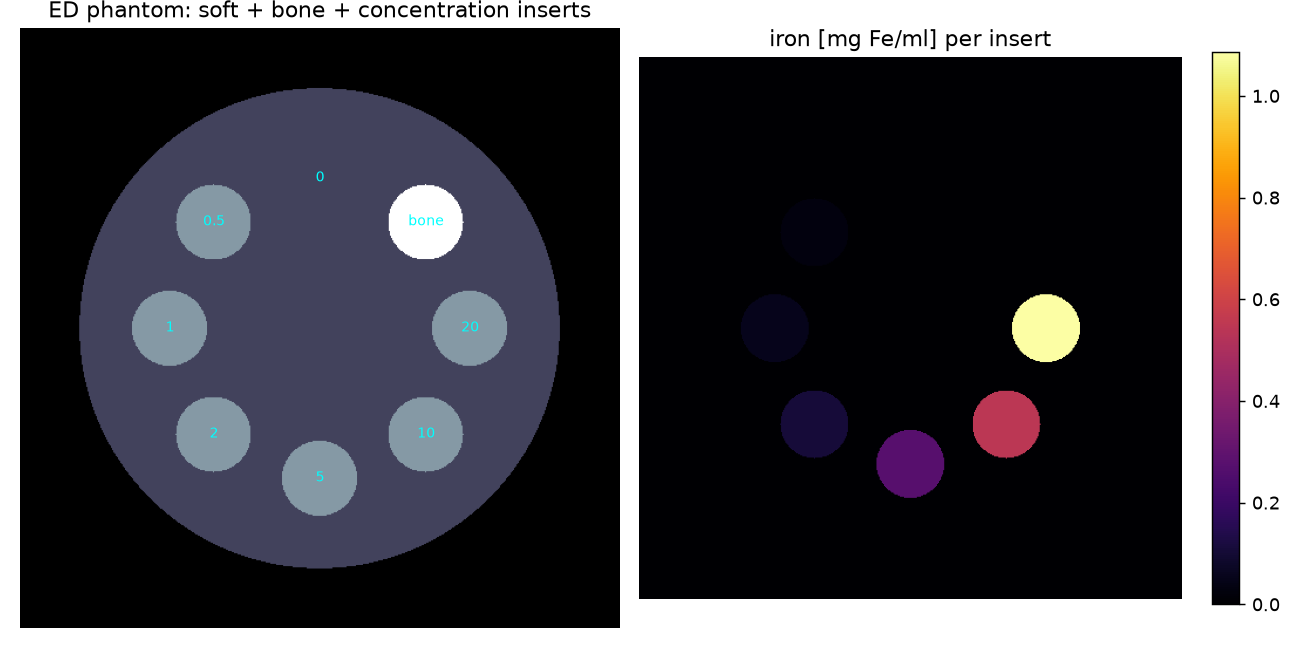
\includegraphics[width=0.42\linewidth]{phantom_axial.png}
\caption{Axial slice of the rabbit-scale phantom: a soft-tissue cylinder with the
seven iron-concentration inserts on a ring and a cortical-bone rod (beam-hardening
source).}
\label{fig:phantom}
\end{figure}

\subsection{X-ray simulation}
We image the phantom with the CONRAD standard polychromatic spectrum
($90\,\mathrm{kVp}$, mean energy $55.4\,\mathrm{keV}$; Fig.~\ref{fig:spectrum}) in a
standard C-arm cone-beam geometry with $500$ projections over a short scan. The
base-material path lengths are obtained analytically by ray tracing the phantom,
and combined polychromatically per energy through the Beer--Lambert law. We
simulate two detectors. The EID integrates the transmitted spectrum weighted by
photon energy; the PCD sorts photons into three energy bins with thresholds at
$37.5$ and $50\,\mathrm{keV}$, which an ideal-observer analysis identified as
near-optimal for this task, and combines the bins with matched-filter weights.
Quantum noise is Poisson at $70{,}000$ photons per pixel, applied per energy on the
photon counts \emph{before} energy weighting or binning; this is important, because
the variance of an energy-integrated signal is $\sum_E E^2 n_E$, which a single
Poisson draw on the summed signal would not reproduce.

\begin{figure}[ht]
\centering

\includegraphics[width=0.6\linewidth]{spectrum.png}
\caption{CONRAD polychromatic C-arm spectra (tungsten anode with characteristic
lines) at three tube voltages. The $90\,\mathrm{kVp}$ spectrum is the study
standard.}
\label{fig:spectrum}
\end{figure}

\subsection{Reconstruction}
Each noisy sinogram is reconstructed with filtered back-projection on a
$0.5\,\mathrm{mm}$ isotropic grid. Beam-hardening correction is applied in a water
precorrection variant that we switch on and off. Figure~\ref{fig:recon} shows an
example sinogram and reconstruction. The GPU back-projector used here required a
fix to the CONRAD OpenCL kernel, which never received the reconstruction pixel
spacing; the corrected kernel matches the CPU reference to $\sim\!10^{-5}$ and is
roughly $850\times$ faster, and has been contributed upstream.

\begin{figure}[ht]
\centering
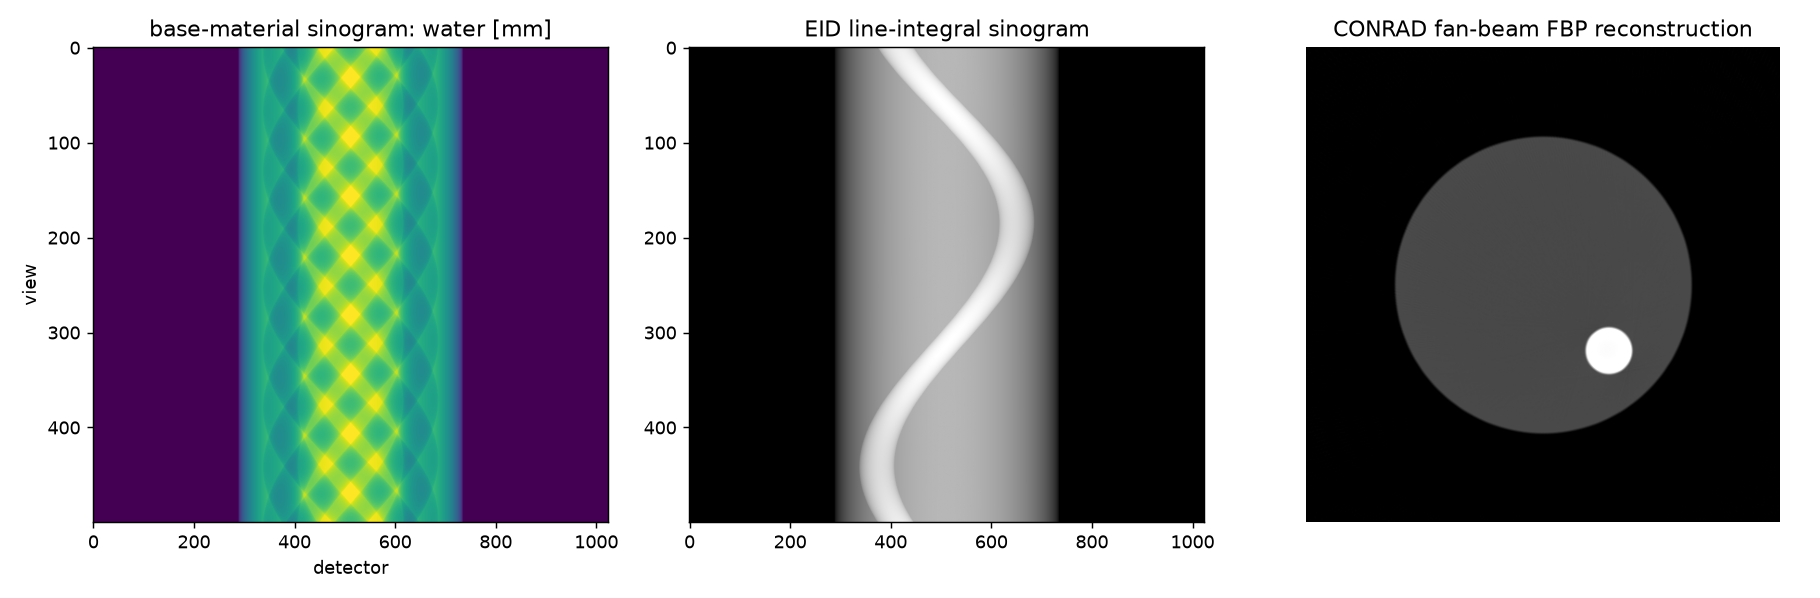
\includegraphics[width=0.92\linewidth]{native_pipeline.png}
\caption{Example of the CONRAD-native pipeline: base-material sinogram (left),
energy-integrated line-integral sinogram (center), and fan-beam FBP reconstruction
(right).}
\label{fig:recon}
\end{figure}

\subsection{Evaluation}
We score detectability with two metrics. The iron contrast $\Delta$HU is the mean
insert value minus a local annular background (which shares the insert's cupping and
streak level), corrected by subtracting the zero-iron insert so that only iron
remains. The CNR is that contrast divided by the background noise measured over
noise realizations. An insert is called detectable when its CNR clears the Rose
criterion (we report both $\mathrm{CNR}\ge 3$ and $\ge 5$). The full factorial is
seven doses $\times$ two detectors $\times$ two beam-hardening states $\times$ $30$
noise realizations. A separate sweep varies the tube voltage
($60$--$120\,\mathrm{kVp}$) and adds hardening filters, to test the spectral
dependence predicted by the photoelectric nature of iron.

\begin{table}[ht]
\caption{Simulation parameters.}
\label{tab:params}
\begin{center}
\begin{tabular}{ll}
\toprule
Parameter & Value \\
\midrule
Spectrum & CONRAD standard, $90\,\mathrm{kVp}$ (mean $55.4\,\mathrm{keV}$), W anode \\
Photons per pixel & $70{,}000$ (Poisson) \\
Geometry & C-arm cone beam, $500$ projections, short scan \\
Source-to-isocenter / detector & $750\,\mathrm{mm}$ / $1200\,\mathrm{mm}$ \\
Field of view & $200\,\mathrm{mm}$ \\
Reconstruction & FBP, $0.5\,\mathrm{mm}$ isotropic voxels \\
Phantom & $110\,\mathrm{mm}$ soft-tissue cylinder + cortical-bone rod \\
Tumor & $8\,\mathrm{cm}^3$ ($r=12.4\,\mathrm{mm}$), iron-loaded \\
Detectors & EID; 3-bin PCD, thresholds $37.5/50\,\mathrm{keV}$ \\
Dose levels & $c_{\mathrm{Fe}} \in \{0.027,\dots,1.086\}\,\mathrm{mg/ml}$ (Table~\ref{tab:dose}) \\
Noise realizations & $30$ per cell \\
\bottomrule
\end{tabular}
\end{center}
\end{table}

\section{RESULTS}
\label{sec:results}

\subsection{Iron contrast and detectability versus dose}
The central result is that SPIONs sit right at the CT detection limit at the
realistic dose. Figure~\ref{fig:dhu} shows iron contrast rising smoothly with
concentration. At the reference $6\,\mathrm{mg}$ dose
($c_{\mathrm{Fe}}=0.54\,\mathrm{mg/ml}$) the contrast is only $3.4\,$HU for the EID
and $4.7\,$HU for the PCD; at twice the dose it reaches $7.1$ and $9.0\,$HU. The
photon-counting detector produces the larger contrast, as expected from its
low-energy weighting.

\begin{figure}[ht]
\centering
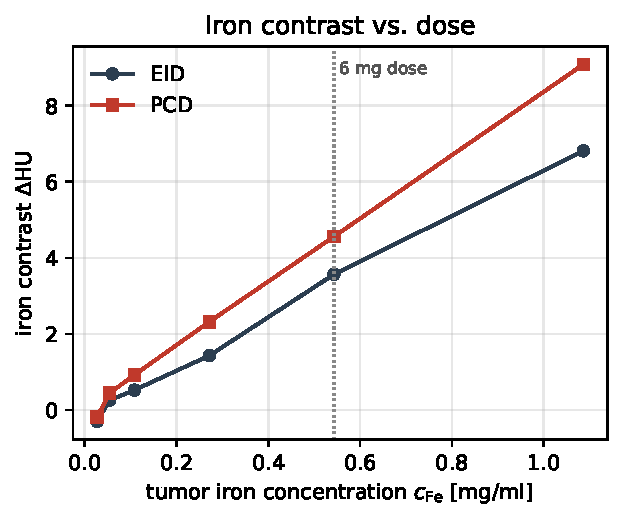
\includegraphics[width=0.58\linewidth]{fig_dhu_vs_conc.pdf}
\caption{Iron contrast $\Delta$HU versus in-tumor iron concentration for the two
detectors (beam-hardening off). The dotted line marks the realistic $6\,\mathrm{mg}$
dose.}
\label{fig:dhu}
\end{figure}

Turning contrast into detectability, Fig.~\ref{fig:cnr} plots CNR against dose with
the Rose lines overlaid. Detectability crosses $\mathrm{CNR}\approx 5$ exactly at
the realistic dose: $5.4$ for the EID and $5.1$ for the PCD. The resulting
detection threshold is $\approx 0.54\,\mathrm{mg\,Fe/ml}$ and, strikingly, it is
the same for all four combinations of detector and beam-hardening correction
(Table~\ref{tab:thresh}). Beam-hardening correction changes iron detectability
negligibly, which is expected: iron contrast is a genuine material signal, not a
cupping artifact.

\begin{figure}[ht]
\centering
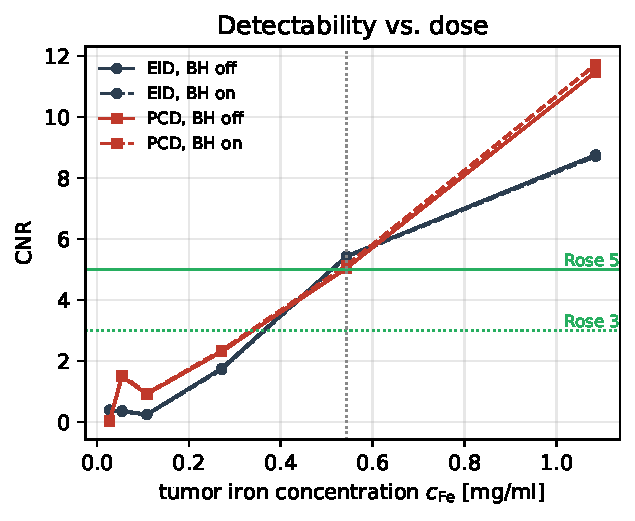
\includegraphics[width=0.58\linewidth]{fig_cnr_vs_conc.pdf}
\caption{CNR versus dose for both detectors, beam-hardening on/off, with the Rose
$3$ and $5$ lines. The realistic dose (dotted) lands on the Rose-$5$ boundary.}
\label{fig:cnr}
\end{figure}

\begin{table}[ht]
\caption{Detection thresholds -- the lowest $c_{\mathrm{Fe}}$ [mg/ml] reaching the
Rose criterion -- per detector and beam-hardening state. The threshold coincides
with the realistic $6\,\mathrm{mg}$ dose and is essentially detector-independent.}
\label{tab:thresh}
\begin{center}
\begin{tabular}{lcc}
\toprule
Condition & Rose $\ge 3$ & Rose $\ge 5$ \\
\midrule
EID, BH off & 0.54 & 0.54 \\
EID, BH on  & 0.54 & 0.54 \\
PCD, BH off & 0.54 & 0.54 \\
PCD, BH on  & 0.54 & 0.54 \\
\bottomrule
\end{tabular}
\end{center}
\end{table}

\subsection{Where the photon-counting advantage appears}
Photon counting is often expected to rescue low-contrast tasks. Here it does, but
only partly. The matched-filter PCD attains its ideal-observer advantage of
$\sim\!1.3\times$ EID CNR at the top dose ($11.5$ vs.\ $8.8$), where the
high-contrast low-energy bin carries enough counts to be useful. At the realistic
dose the two detectors are indistinguishable, because the low-energy bin is
photon-starved through $\sim\!11\,\mathrm{cm}$ of tissue. Figure~\ref{fig:pcd}
shows where iron contrast lives in energy and the near-optimal three-bin
thresholds; the entire spectral gain is concentrated in a band that receives few
transmitted photons.

\begin{figure}[ht]
\centering

\includegraphics[width=0.6\linewidth]{pcd_bins.png}
\caption{Per-energy iron detectability density through the phantom, with the
near-optimal three-bin PCD thresholds ($37.5/50\,\mathrm{keV}$). The contrast lives
where transmitted photons are scarce, which limits the realized PCD gain.}
\label{fig:pcd}
\end{figure}

\subsection{Spectral shaping}
Because iron contrast is photoelectric, it should favor low energy. The tube-voltage
and filter sweep (Fig.~\ref{fig:sweep}) confirms this end-to-end: EID CNR at the top
dose falls monotonically from $9.9$ at $60\,\mathrm{kVp}$ to $7.6$ at
$120\,\mathrm{kVp}$, and the detection threshold improves to
$0.54\,\mathrm{mg\,Fe/ml}$ at $60$--$80\,\mathrm{kVp}$ but degrades to
$1.09\,\mathrm{mg\,Fe/ml}$ at $100$--$120\,\mathrm{kVp}$. Hardening filters move the
spectrum the wrong way; an ideal-observer analysis on the same spectra gives a
$1.34\times$ CNR gain at $60\,\mathrm{kVp}$ and a $0.58\times$ penalty for a
$0.5\,\mathrm{mm}$ tin filter. The practical message is simple: to see iron, use a
soft spectrum.

\begin{figure}[ht]
\centering
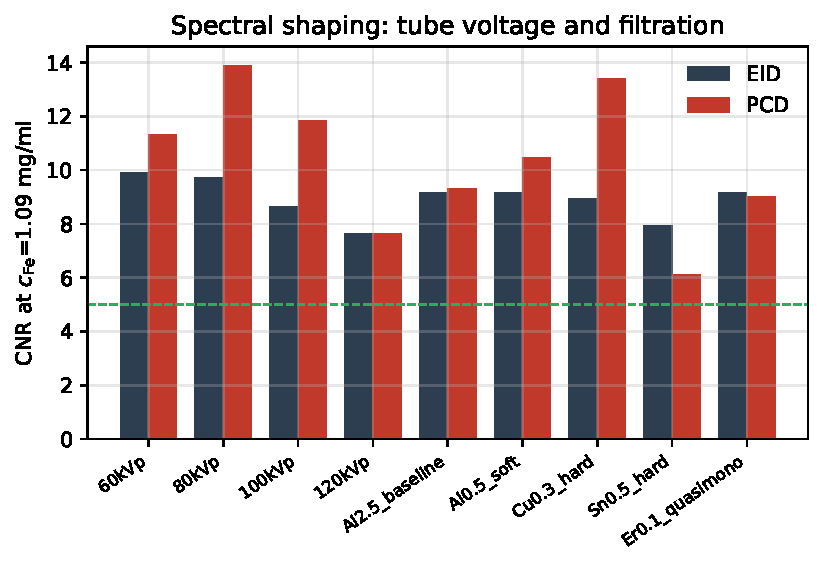
\includegraphics[width=0.75\linewidth]{fig_spectral_sweep.pdf}
\caption{Spectral shaping. CNR at the top dose for both detectors across tube
voltages and added filters. Lower tube voltage helps; hardening filters hurt.
(PCD estimates use fewer noise realizations and are correspondingly noisier.)}
\label{fig:sweep}
\end{figure}

\subsection{Heterogeneous (vascular) uptake}
Real uptake is vascular, not uniform, so we also test a two-compartment tumor in
which the same delivered iron mass is confined to $150\,\mu\mathrm{m}$ vessels
occupying $10\%$ of the tumor volume -- a tenfold local concentration. The decisive
fact is one of scale: a $0.5\,\mathrm{mm}$ voxel is more than three times wider than
a vessel, so each voxel partial-volume-averages many vessels. With mass conserved,
the volume-averaged iron per voxel is therefore unchanged, and the tumor-ROI
contrast is identical to the homogeneous case; our simulation confirms a ROI-mean
iron concentration equal to the homogeneous mean at every voxel size we tested, and
a per-voxel peak that reaches the true tenfold value only as the voxel shrinks
toward the vessel size (Fig.~\ref{fig:studyb}). Two second-order effects that the
homogeneous model omits both prove negligible here: the beam-hardening
nonlinearity from concentrating iron into vessels is below $10^{-3}\,$HU even at
five times the reference dose, because iron is such a small perturbation of the
line integral; and although the per-voxel vessel count is binomial and adds
substantial texture ($\sim\!90\%$ relative per-voxel at $0.5\,\mathrm{mm}$, with
$\sim\!11$ vessels per voxel), this averages out over the tumor ROI. In short, at
realistic resolution and dose, vascular uptake is CT-indistinguishable from
homogeneous uptake, and the simpler homogeneous model is adequate for the
detectability question.

\begin{figure}[ht]
\centering
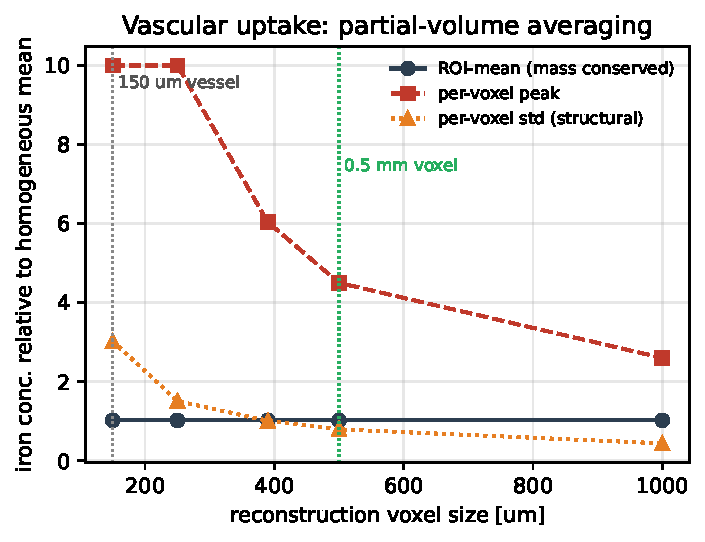
\includegraphics[width=0.58\linewidth]{fig_study_b.pdf}
\caption{Vascular uptake and partial-volume averaging. The ROI-mean iron
concentration is invariant (mass conservation), while the per-voxel peak approaches
the resolved tenfold value only as the voxel shrinks toward the
$150\,\mu\mathrm{m}$ vessel size; at the $0.5\,\mathrm{mm}$ CT voxel the vessels are
unresolved.}
\label{fig:studyb}
\end{figure}

\section{DISCUSSION}
\label{sec:discussion}

The picture that emerges is coherent. At biologically realistic loading, SPIONs
deposit little iron, that iron produces only a few Hounsfield units of contrast,
and the resulting CNR lands on the Rose criterion rather than comfortably above it.
The reference $6\,\mathrm{mg}$ dose is therefore borderline-visible: detectable in
principle at low noise and a soft spectrum, but not a robust, everyday finding. To
put the number in context, the top-end iron concentration we study
($\sim\!1\,\mathrm{mg\,Fe/ml}$) is still about an order of magnitude below typical
iodinated-contrast enhancement, so it is unsurprising that detectability is marginal.

Which knob helps most? Not the detector, and not beam-hardening correction. A
three-bin photon-counting detector with optimal energy weighting delivers its
theoretical $\sim\!1.3\times$ advantage only once the dose is high enough for the
low-energy bin to matter; at the realistic dose that bin is photon-starved and the
advantage vanishes into noise. The lever that does move the threshold is the
spectrum: a softer beam (lower kVp, no hardening filtration) raises iron contrast
where it is photoelectric. This is consistent across the ideal-observer analysis,
the full reconstruction pipeline, and the physical intuition.

We state the limitations candidly, because they bound the claim. The study is a
simulation with idealized, ideal-energy detectors and no scatter or patient motion.
The phantom is a round, geometric, rabbit-scale cylinder rather than real rabbit
anatomy -- no standard digital rabbit phantom exists -- so beam hardening and
scatter are idealized; results are reported for a central slice. Soft tissue is a
water proxy, since CONRAD ships no ICRU-44 soft-tissue definition, and the residual
bone-streak bias is suppressed but not eliminated by the local-background and
zero-iron subtraction. The homogeneous-uptake assumption is relaxed by the vascular
model of Sec.~\ref{sec:results}, which shows that sub-resolution vessels do not
change detectability at the same total dose; what remains is the absence of true
anatomy and a full three-dimensional study. As a bridge to that study, we have
already reconstructed the acquisition geometry of a real post-mortem rabbit C-arm
scan from the RabbitCT benchmark\cite{Rohkohl2009} -- a $745\,\mathrm{mm}$
source-to-isocenter, $1196\,\mathrm{mm}$ source-to-detector short scan of $496$
projections over $198^\circ$ -- by decoding its projection matrices. Casting rays
through the reference rabbit volume with that geometry yields cone-beam digital
radiographs in which the skull and cervical spine appear correctly and rotate with
view angle, validating the extracted geometry end to end; inserting an
$8\,\mathrm{cm}^3$ SPION tumor makes it project as a localized signal that tracks
the anatomy (Fig.~\ref{fig:rabbit}). A full polychromatic cone-beam FDK
detectability study on this phantom is the immediate next step.

\begin{figure}[ht]
\centering
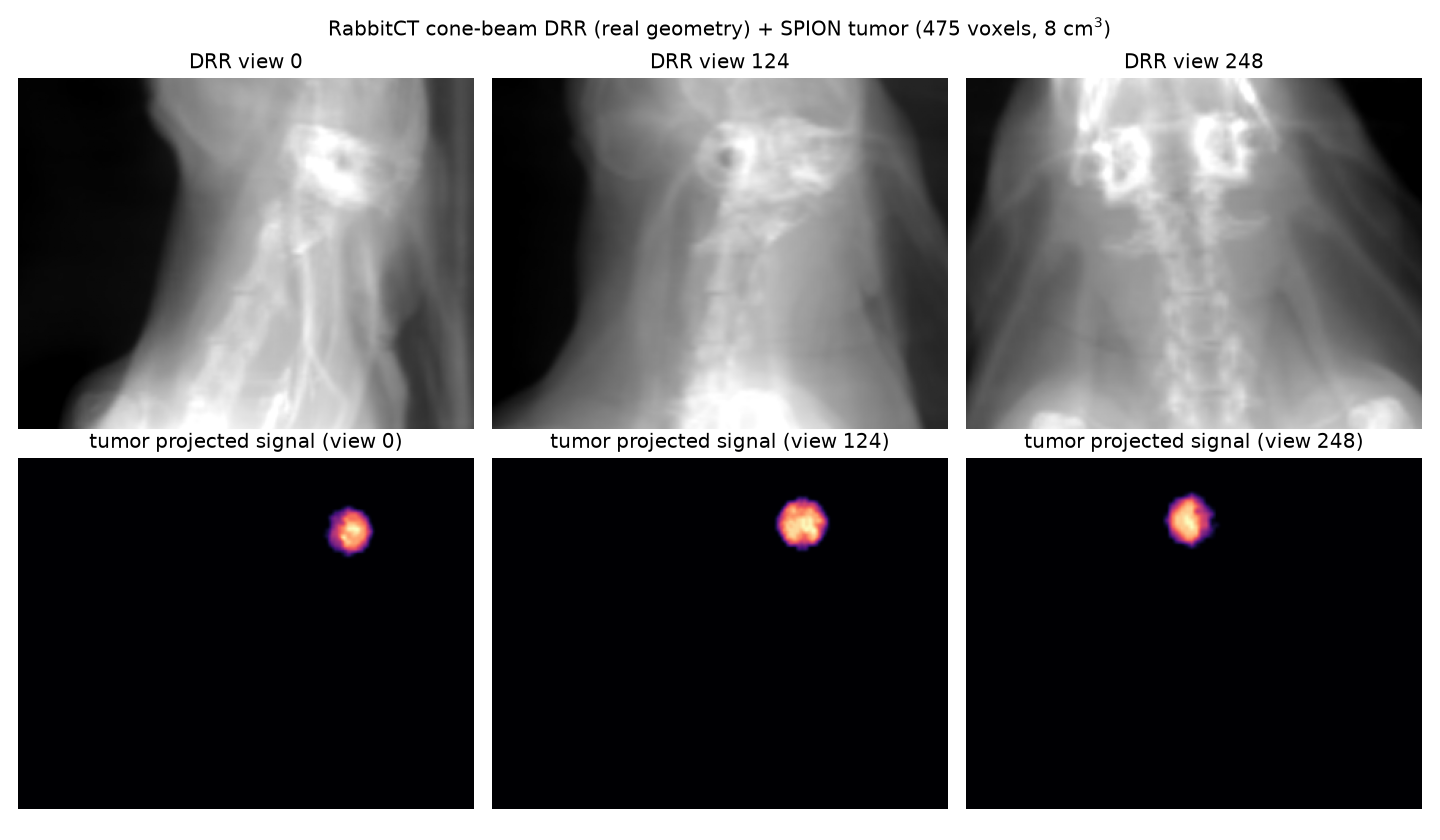
\includegraphics[width=0.98\linewidth]{rabbit_drr_tumor.png}
\caption{Toward a three-dimensional study in real anatomy. Top: ray-driven
cone-beam digital radiographs of the post-mortem RabbitCT rabbit at three view
angles, using the C-arm geometry ($745/1196\,\mathrm{mm}$, $496$ views over
$198^\circ$) decoded from the benchmark's projection matrices. Bottom: the
projected signal of an inserted $8\,\mathrm{cm}^3$ SPION tumor, which tracks the
anatomy across views.}
\label{fig:rabbit}
\end{figure}

\section{CONCLUSION}
\label{sec:conclusion}

Are magnetic nanoparticles visible in CT? At realistic biological loading, only
barely. Our simulation places the detection limit at
$\approx 0.54\,\mathrm{mg\,Fe/ml}$ -- essentially the reference $6\,\mathrm{mg}$
SPION dose -- with an iron contrast of a few Hounsfield units and a CNR on the Rose
boundary. Neither photon counting nor beam-hardening correction lowers that limit
at realistic dose; a soft spectrum is the most effective lever. For image-guided
nanoparticle therapy this means that routine CT confirmation of SPION delivery is
feasible only at the upper end of realistic loading and with a spectrum tuned for
iron. The path forward is experimental validation against phantom and \emph{ex
vivo} measurements, a heterogeneous (vascular) uptake model, and a full
three-dimensional anatomical study; all of the simulation machinery used here,
including GPU-native spectral detectors and noise generators contributed to CONRAD,
is openly available to support that work.

\section*{Code and data availability}
The complete simulation pipeline, intermediate results, and figure sources are
public, with an audit dashboard at \url{https://akmaier.github.io/SPIONvsXRay/}. The
project is MIT-licensed; the GPU OpenCL detector, noise-generator, and
back-projector contributions have been upstreamed to CONRAD.

\acknowledgments
This work builds on the CONRAD framework of the Pattern Recognition Lab, FAU
Erlangen-N\"urnberg. The nanoparticle formulation and dose grounding are provided by
the SEON group.

\begin{thebibliography}{9}
\bibitem{Maier2013} A.~Maier et al., ``CONRAD -- a software framework for cone-beam
imaging in radiology,'' \emph{Medical Physics} \textbf{40}(11), 111914 (2013).
\bibitem{Heinen2026} L.~Heinen et al., ``PAA-coated magnetite SPION clusters for
magnetic drug targeting,'' \emph{Ultrasonics Sonochemistry} \textbf{130}, 107876
(2026).
\bibitem{Rose} A.~Rose, \emph{Vision: Human and Electronic}, Plenum Press, New York
(1973).
\bibitem{Willemink2018} M.~J.~Willemink et al., ``Photon-counting CT: technical
principles and clinical prospects,'' \emph{Radiology} \textbf{289}(2), 293--312
(2018).
\bibitem{Rohkohl2009} C.~Rohkohl, B.~Keck, H.~G.~Hofmann, and J.~Hornegger,
``Technical Note: RabbitCT -- an open platform for benchmarking 3D cone-beam
reconstruction algorithms,'' \emph{Medical Physics} \textbf{36}(9), 3940--3944
(2009).
\bibitem{Tapiovaara1985} M.~J.~Tapiovaara and R.~F.~Wagner, ``SNR and DQE analysis
of broad spectrum X-ray imaging,'' \emph{Phys. Med. Biol.} \textbf{30}(6), 519--529
(1985).
\bibitem{Salmon2011} J.~K.~Salmon et al., ``Parallel random numbers: as easy as
1,2,3,'' in \emph{Proc. SC'11}, ACM (2011).
\bibitem{Hormann1993} W.~H\"ormann, ``The transformed rejection method for
generating Poisson random variables,'' \emph{Insurance: Mathematics and Economics}
\textbf{12}(1), 39--45 (1993).
\bibitem{Maier2019} A.~Maier et al., ``A gentle introduction to deep learning in
medical image processing,'' \emph{Z. Med. Phys.} \textbf{29}(2), 86--101 (2019).
\end{thebibliography}

\end{document}
